\beginsong{Ungezählte Male}[wuw={trenk (Alo Hamm)}, bo={334}]

\markboth{\songtitle}{\songtitle}

\beginverse
\endverse

\centering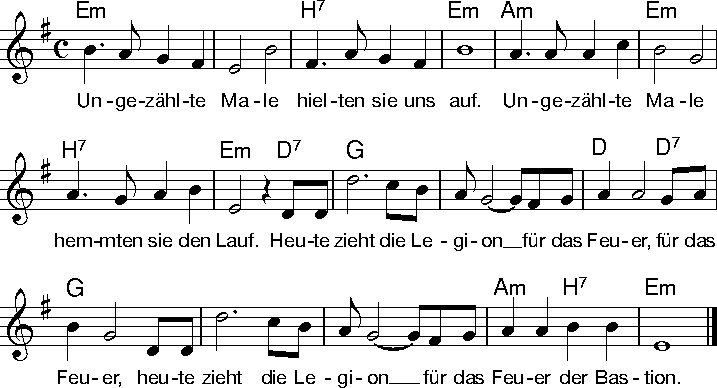
\includegraphics[width=1\textwidth]{Noten/Lied089.pdf}	

\beginverse
\[Em]Dunkle Männer kamen \[H7]lammfelleinge\[Em]hüllt.
\[Am]Was sie auch ver\[Em]sprachen, \[H7]wurde nie er\[Em]füllt.
\endverse

\beginchorus
\[D7]Heute \[G]zieht die Legion für das \[D]Feuer, \[D7]für das 
\[G]Feuer, heute zieht die Legion für das \[Am]Feuer \[H7]der Ba\[Em]stion.
\endchorus

\beginverse
^Licht in dunklen Tagen, ^junge Gen'ra^tion.
^Auf die Barri^kaden ^geist'ger Rebell^ion. 
\endverse

\renewcommand{\everychorus}{\textnote{\bf Refrain (wdh.)}}
\beginchorus
\endchorus

\endsong
\beginscripture{}

\endscripture

\begin{intersong}

\end{intersong}
